% Section 8: Summary, Q&A, and Literature (Slides 61-63)

% Slide 61: Online Lectures
\begin{frame}{ویدیوهای آموزشی آنلاین}{\lr{Online Lectures}}
  \begin{columns}[T]
    \begin{column}{0.48\textwidth}
      \begin{itemize}
        \setlength{\itemsep}{10pt}
        \item \textbf{اهمیت ویدیوهای مکمل:}
        \begin{itemize}
          \setlength{\itemsep}{5pt}
          \item برای حل تمرین‌های عملی هفتگی و آزمون پایان‌ترم، مشاهده ویدیوهای برخط درس الزامی است.
          \item بررسی جزئیات پیاده‌سازی و شبیه‌سازی الگوریتم‌ها با مثال‌های متعدد
        \end{itemize}
      \end{itemize}
    \end{column}
    \begin{column}{0.48\textwidth}
      \begin{center}
        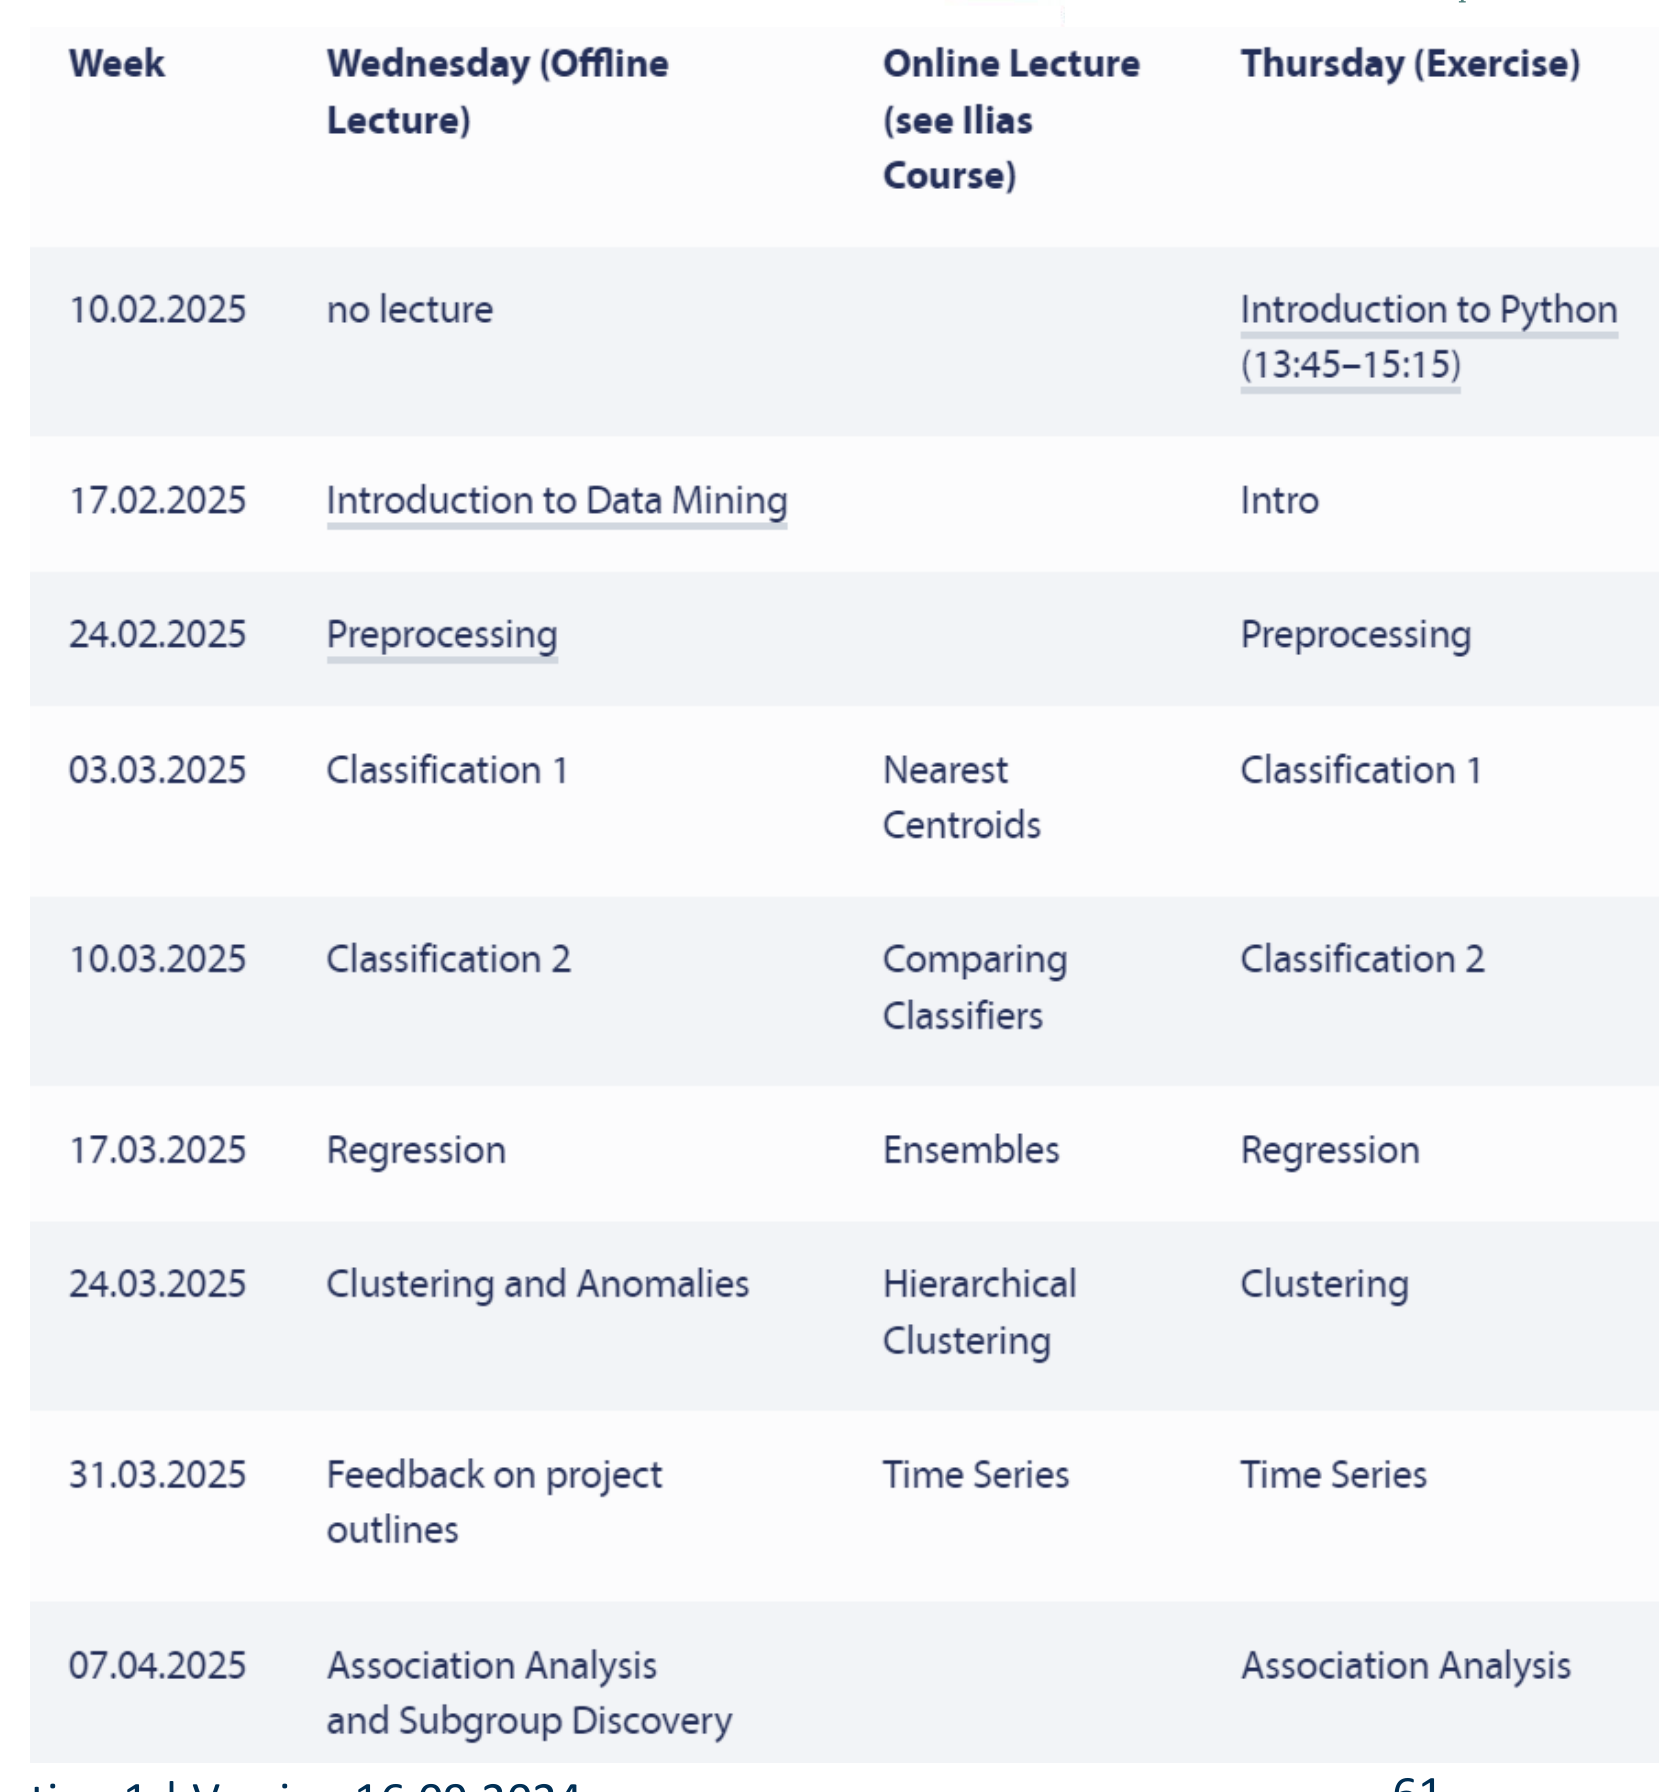
\includegraphics[width=\textwidth,height=5.2cm,keepaspectratio]{images/slide61_online_lectures.png}
      \end{center}
    \end{column}
  \end{columns}
\end{frame}

% Slide 62: Questions?
\begin{frame}{پرسش و پاسخ}{\lr{Questions?}}
  \begin{center}
    
\includegraphics[width=0.65\textwidth,height=5.2cm,keepaspectratio]{images/slide62_questions.png}
  \end{center}
\end{frame}

% Slide 63: Literature
\begin{frame}{منابع و مراجع این مجموعه اسلاید}{\lr{Literature for this Slideset}}
  \begin{columns}[c]
    \begin{column}{0.62\textwidth}
      \begin{itemize}
        \setlength{\itemsep}{7pt}
        \item \begin{latin}\small
          Pang-Ning Tan, Michael Steinbach,\\
          Anuj Karpatne, Vipin Kumar:\\[2pt]
          \textbf{Introduction to Data Mining}.\\
          2nd Edition. Pearson.
        \end{latin}
        \vspace{0.1cm}
        \item \textbf{فصل‌های مرتبط در کتاب:}
        \begin{itemize}
          \setlength{\itemsep}{3pt}
          \item \textbf{فصل ۳: طبقه‌بندی} \lr{(Chapter 3: Classification)}
          \begin{itemize}
            \item بخش ۳.۳: طبقه‌بند درخت تصمیم \lr{(Decision Tree)}
            \item بخش ۳.۴: بیش‌برازش \lr{(Overfitting)}
          \end{itemize}
          \item \textbf{بخش ۶.۱۰.۶: جنگل‌های تصادفی} \lr{(Random Forests)}
        \end{itemize}
      \end{itemize}
    \end{column}
    \begin{column}{0.34\textwidth}
      \begin{center}
        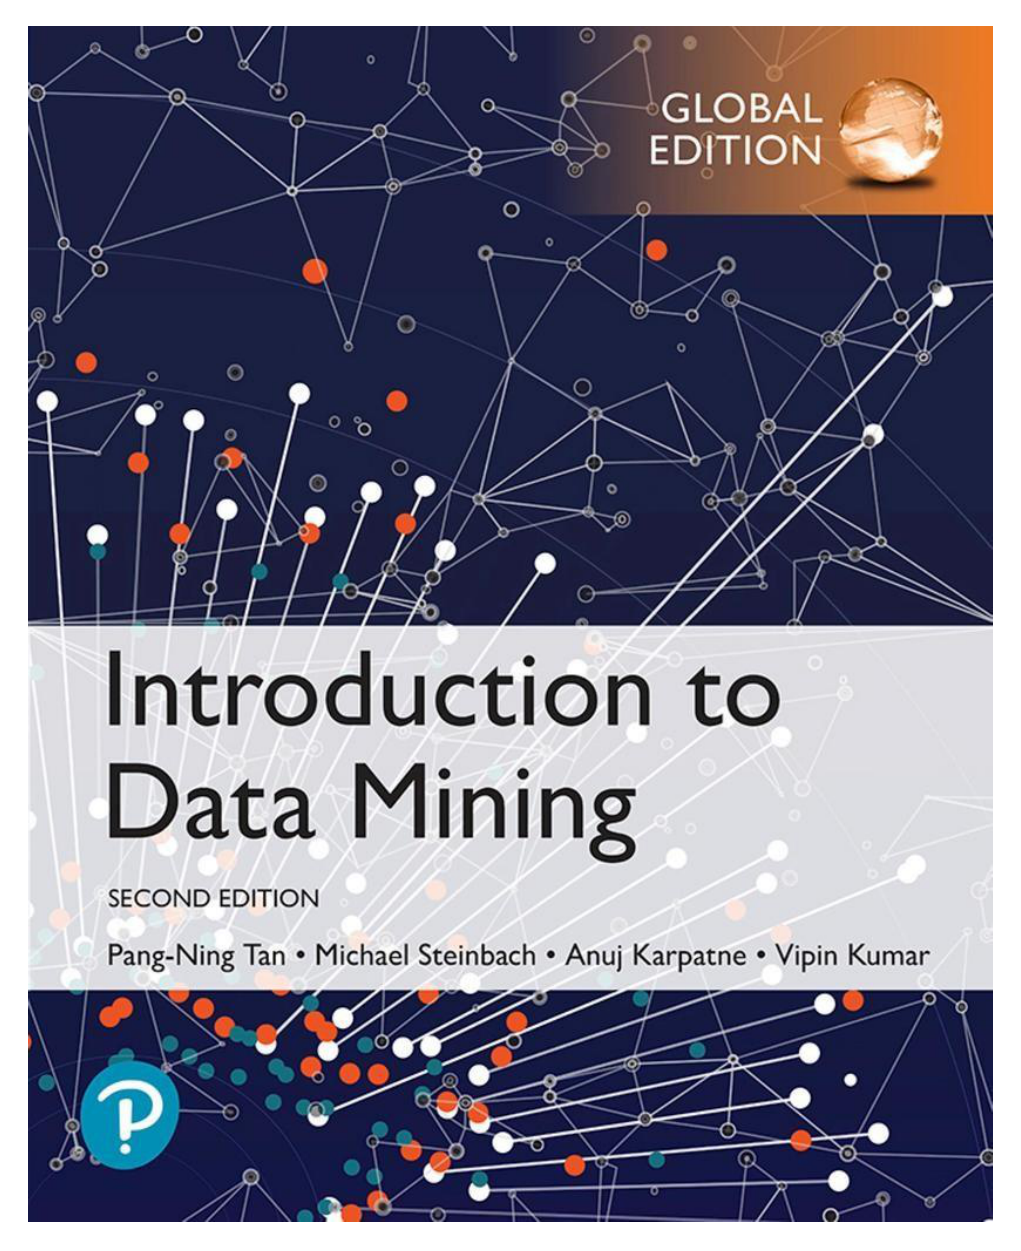
\includegraphics[width=0.88\textwidth,height=4.6cm,keepaspectratio]{images/slide63_literature.png}
      \end{center}
    \end{column}
  \end{columns}
\end{frame}
